
\chapter{Conclusions and Future Work}

The workflow of the ttDilepKinFit method, explained in section \ref{app}, needs to be changed so that it is easier and more effective to parallelize its execution. Currently, the variation is applied for each jet/lepton combination, dilep is executed, the results are treated (and the probability of the reconstruction is calculated) and the Higgs boson is reconstructed.

The best approach is to create a data set with all the jet/lepton combinations and all the respective variations. Then, execute dilep with all the elements on the data set and store all the results with the associated element of the data set. Note that the number of dilep executions per event will be equal to the number of jet/lepton combination times the number of variations per combination. Finally, iterate through all of the results, reconstruct each Higgs boson and calculate the respective probability for each element of the first data set. Figure \ref{fig:pipeline} represents the current and the alternative workflows.

\begin{figure}[!htp]
	\begin{center}
		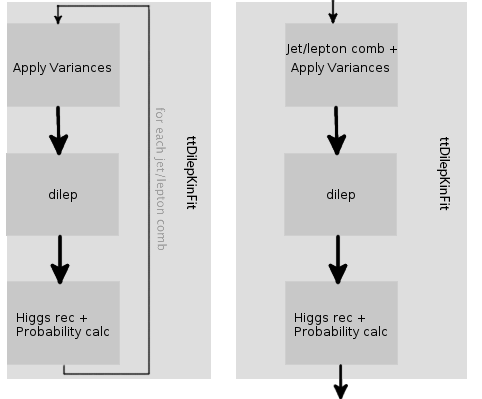
\includegraphics[scale=0.5]{../../common/img/pipeline.png}
		\caption{Current workflow (left) vs alternative workflow (right) of the ttDilepKinFit method.}
		\label{fig:pipeline}
	\end{center}
\end{figure}

This approach offers (theoretically) the possibility of having three distinct parallel tasks. The first would be the jet/lepton combination and variance calculations. The second, would be the dilep executions, which are independent, it is only needed to merge the results after. The third would be the final iteration through the results of each dilep execution and respective Higgs reconstruction. However, these three parallel tasks are dependent on each other. 

To ease the cost of this dependency a queue-based approach will be tested. As the first data set is constructed, its elements can be provided to the next parallel task, where dilep is executed. As soon as the results from dilep are available they can be passed to the third parallel region and the Higgs boson can be reconstructed. In theory, this will decrease the execution time, relative to a strict implementation, where all the parallel tasks are being executed at the same time after an initial latency.

After this stage, an implementation of the kinematical reconstruction (dilep), which is the most time consuming task in the Loop method, and it tends to increase even more with the number of variances specified, will be attempted on both GPUs and Xeon Phi. The efforts will be towards obtaining the most optimal hybrid (i.e., also using the CPU) implementation possible. The performance will be measured and compared between these devices and the bottlenecks identified.

Finally, an implementation using the OpenACC and GAMA frameworks will be tested, relatively to the previous optimized implementations, in terms of performance but also considering the development time and usability of these tools.

\newpage
